\documentclass[a4paper]{article}
%\usepackage{ucs}
\usepackage[T1]{fontenc}
\usepackage[utf8x]{inputenc}
\usepackage[magyar]{babel}
\usepackage{graphicx}
\usepackage{url}
\usepackage{indentfirst}


%A kettő közül az egyik megjegyzésbe teendő.
%az utasítáasokban nem lehet \verb, vázlatnál érdemes a4paper-t használni
\newcommand{\csakvazlat}[1]{#1} \newcommand{\csakeloadas}[1]{}
%\newcommand{\csakeloadas}[1]{#1} \newcommand{\csakvazlat}[1]{}
%Az előadás sortörései 25%-os nagyításhoz jók.

\begin{document}
\title{Rövid \LaTeX\ összefoglaló}
\author{Horváth Árpád\\ÓE, AREK}
\maketitle

\section*{Irodalom}
A \LaTeX\ használatához magyar nyelvű felhasználóknak szinte nélkülözhetetlen
\emph{ Wettl--Mayer--Sudár: \LaTeX\ kezdőknek és haladóknak} című könyve
vagy a ,,Latex2e 78 percben'' interneten elérhető dokumentum. 
%További hasznos információk érhetőek el a \url{www.arek.uni-obuda.hu/harp/latex} honlapomról.

\section*{Bevezető}
\addcontentsline{toc}{section}{Bevezető}

A \LaTeX\ fájl egy sima szöveges fájl, mely sokmindenben a html-hez hasonlít,
de végcélja egy nyomtatott dokumentum készítése.
Vannak hozzá olyan szövegszerkesztők, amelyeknél a végeredményt rögtön látom,
de mivel rengeteg különböző (akár házilag írt) csomagot használhatunk hozzá,
ezért lehetetlen, hogy mindet ismerje.

A jelenlegi jegyzetben csak a legalapvetőbb dolgok
vázlatszerű összefoglalására szorítkozom.
 A célom tulajdonképpen, hogy egy kezdő felhasználónak
kis segítséget nyújtsak.

\csakeloadas{\newpage}

A \LaTeX-et érdemes használni, 
\begin{itemize}
\item ha sok programrészlet, táblázat vagy képlet van a dokumentumban, 
\item ha tipográfiai ismeretek nélkül szép kivitelű kiadványt szeretnénk létrehozni
	(ajánlom szakdolgozathoz),
\item vagy ha egy nagyobb kiadvány számára egységes kinézetet szeretnénk biztosítani (Ez könnyen megoldható akkor is, ha  egy könyvet több szerző ír.),
\item ha többféle operációs rendszert használunk.
\end{itemize}

\csakeloadas{\newpage}


\csakeloadas{
A \LaTeX\ fájlt különböző programokkal fordíthatjuk le dvi majd PostScript illetve PDF formátumokba. Ezek
bármely gyakoribb gépen és operációs rendszeren
megnézhetőek, és pont úgy néz ki mint a másikon.
A fordítóprogramok szintén sokféle operációs rendszer alatt léteznek.
(A Windowson, a legtöbb UNIX-on, linuxon, OS/2-n, a Macintosh operációs rendszerén, DOS alatt \dots)

\subsection*{Rövid története}
\begin{itemize}
\item  A \TeX\ szövegformázó nyelv 
(1977-ben írta Donald E.Knuth stanfordi matematikus):
 neve a \emph{techné = \(\tau\epsilon\chi\nu\eta\) = művészet}
 görög szóból ered, teh-nek ejtendő.

\item A \LaTeX\ makrógyűjtemény (Leslie Lamport 1980-as évek eleje)

\item Az AMS-\LaTeX\ és a \LaTeX

\item A \LaTeX3 fejlesztése (1989-től) és a \LaTeXe (1994)
\end{itemize}
}%csakeloadas


\section{A \LaTeX\ alapgondolata}

 Nem a szerző dolga, hogy a kinézettel foglalkozzon!
Hanem a tipográfusé. Ezt a szerepet tölti be a \LaTeX. 

 A szerző dolga, hogy tudja, hogyan épül fel a mű. (fejezetek, kiemelés, mit kell sorszámozni stb.)

 A kinézet és a tartalom szétválasztása azért is előnyös, mert később több cikk, fejezet könnyen összefűzhető.
Könnyen átvihető  másfajta formátumba. (Például más folyóirat közli.)


\section{A \LaTeX\ dokumentum}

\subsection{A \LaTeX\ dokumentum felépítése}

\begin{verbatim}
 \documentclass[a4paper]{article}
    Preambulum 
 \begin{document}
    A dokumentum szövege
 \end{document}
\end{verbatim}

A bekezdések elválasztása üres sorral;
a szavak elválasztása minimum egy szóköz, tabulátor
vagy újsor karakterrel történik.

\paragraph{Utasítások} A dokumentum szövegében $\backslash$-el kezdődő utasítások is vannak
 A [\,] zárójel opcionális,
a \{\} zárójel kötelező argumentumot jelöl. 

Példa: \verb+\framebox[20mm][c]{középre}+ egy 20mm széles keretbe zárja a
középre szót, és középre (c) rakja vizszintesen. Íme:
\framebox[20mm][c]{középre}
 
\paragraph{A dokumentumosztályok}
 Lehetnek: article (cikk), book (könyv), report (értekezés), 
  slides (írásvetítőfólia), letter (levél), proc (konferencia-kiadvány),
  amsldoc (programdokumentum)

 Az article osztály opcionális argumentumai: a4paper, a5paper, b5paper,
  11pt, 12pt, twocolumn, twoside

\paragraph{A csomagok}
 A \verb+\usepackage[opc]{csomag}+ utasítással hívhatóak be
a \LaTeX\ képességeit kibővítő csomagok. Ezek mindig a preambulumba kerülnek.

 Példák: \verb+\usepackage[magyar,english,german,croatian]{babel}+\\
betöltésekor a \LaTeX\ ismerni fogja a fenti helyesírásokat.
 \par Ábrák beillesztéséhez szükség van a graphics vagy graphicx
csomagra, azaz pl. \verb+\usepackage{graphicx}+ kell a preambulumba.

\paragraph{A fejezetek szintjei csökkenő sorrendben (article)}
\begin{verbatim}
\section{}, \subsection{},  \subsubsection{},\\
\paragraph{}, \subparagraph{} 
\end{verbatim}

A book és report dokumentumosztályban létezik még a
part\{\} és a chapter\{\}. Ezek a legmagasabbak.\\

\paragraph{Speciális jelentésű karakterek}
 A $\backslash$ karakter parancsszó kezdetét jelöli.\\ 
 A $\backslash\backslash$ sortörést csinál.\\
 A \{ \} közötti részek egy blokknak számítanak.\\
 A \% utáni rész a sorban megjegyzés.\\
 A \~{ } jel nem eltörhető szóközt jelöl.\\
 A \^{ }, \_, \$, \# és \& karaktereket lásd később.

\csakeloadas{
\newpage
\subsection{Egyéb}
\begin{itemize}
\item oldalszámok 
\item a soknyelvűség és a babel
  \begin{itemize}
    \item tételszerű környezetek és ábrák sorszámozása
      (elöl a szám, utána pont)
    \item magyar elválasztás
    \item egyszerre akár többféle nyelv használata
  \end{itemize}
\item a magyar fontok
  \begin{itemize}
	\item inputenc, hogy ne legyen \~o és \^u az 
		ő és ű helyett
	\item t1enc, hogy az ékezetes karaktereket jól kezelje elválasztáskor
  \end{itemize}
\end{itemize}
}%csakeloadas


\newpage
\subsection{Egy magyar dokumentum kerete}

\begin{verbatim}
 \documentclass[a4paper]{article}
	
   %Ezek a magyar nyelvhez kellenek:
   \usepackage[T1]{fontenc}
   \usepackage{ucs}
   \usepackage[utf8x]{inputenc}
   \usepackage[magyar]{babel}

   %A preambulumba jöhetnek még egyéb csomagok,
   %utasítások definíciói, szövegterület méretére
   %vonatkozó beállítások.

 \begin{document}

   \title{Micimackó kuckója}
   \author{Milne}
   \date{}
   \maketitle %Ez az utasítás írja ki a címet.

   \section{Füles kuckója}
      \subsection{Szépen indult a nap}
      ...
   \tableofcontents %tartalomjegyzék
 \end{document}
\end{verbatim}
\vspace{3ex}

\subsection{Mértékegységek és hosszúságparancsok}
 \paragraph{Rögzített} mm, cm, in (inch), pt (pont), dd, cc, pc, sp, bp (a pont rokonai)
 \paragraph{Betűmérettel kapcsolatos} ex, em (az éppen aktuális x magassága ill. az M szélessége), mu ($\frac1{18}$em matematikai módban)
 \paragraph{Végtelen rugalmas egység} fill
 \paragraph{A dokumentum méreteihez igazodó hosszúságparancsok}
	\verb+\textwidth+, \verb+\linewidth+, \verb+\marginparwidth+ \dots

\vfill
Erre is jók a betűmérettel kapcsolatos egységek:

\def\bmf{B\lower-.7ex\hbox{M}F\@}

\bmf\ {\Huge \bmf\ \scriptsize\bmf\  } \emph{\bmf} \texttt{\tiny\bmf} \textbf{\bmf}


\section{A fordítástól az olvasásig}

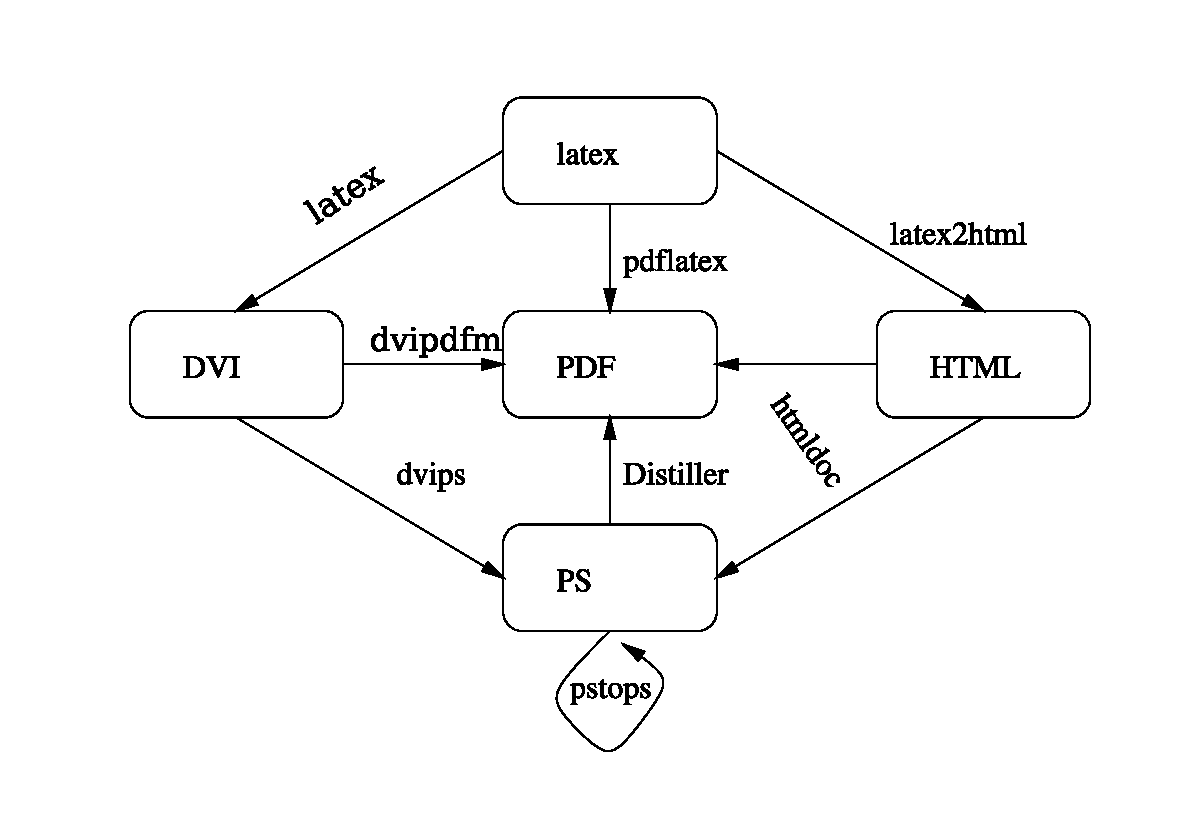
\includegraphics[width=\linewidth]{latex2}


A \LaTeX\ a \verb+latex {fájlnév}+ lefuttatásakor dvi (device independent = eszközfüggetlen) kiterjesztésű fájlt hoz létre.
 
 Ebből \verb+dvips {fájlnév} -o+ paranccsal nyerhetjük a nyomdászok által kedvelt .ps (PostScript) fájlt.

 A PDF (Portable Document Format) formátumába közvetlenül a pdflatex
paranccsal fordíthatunk.
 
 Html formátumba pedig a html2latex (unixos) programmal. 
Ez a képletekből png vagy gif képeket csinál.


\subsubsection*{Hogyan olvasható?}
\begin{center}
\begin{tabular}{|l|c|c|}
\hline
Fájl típus& UNIX alatt& windows alatt\\
\hline \hline
PDF	&evince, acroread&Acrobat Reader\\
\hline
HTML    & Firefox, Opera, lynx, w3m\dots &Firefox, IE\dots\\
\hline
DVI	&	evince, xdvi&	view\\
\hline
PostScript&evince, gv&{Ghostview + GhostScript}\\
\hline
\end{tabular}
\end{center}

Ezek közül - tudtommal - egyedül az Internet Explorer ,,fizetős'' termék.
A html2latex-ről valamint a ghostscript eléréséről és pár hasznos
webes címről bővebb anyag a wikipédián található:
\url{http://hu.wikipedia.org/wiki/LaTeX}

\section{Ábrák}
\subsection{Ábrák beillesztése}
\verb+\includegraphics{grafikus_fajl}+ beilleszti a
\verb+grafikus_fajl.kit+
 ábrát. pdflatex esetén a ,,kit'' kiterjesztés lehet pl. PDF, JPG, a sima latex
esetén EPS (Encapsulated Postscript) és pár más.
Ehhez be kell tölteni a graphicx csomagot. Ezzel a csomaggal rengeteg
hasznos opció is elérhetővé válik. Egy példa.

\verb+\includegraphics[width=0.8\textwidth, angle=40]{grafikus_fajl}+

\subsection{Ábrák készítése}
\begin{itemize}
\item grafikus parancsokkal (\verb!peldak/tikz_peldak.tex!)
\item az Inkscape többplatformos vektrografikus szerkesztővel PDF és
PostScript formátumba is menthetünk
\item xfig-gel (UNIX): beilleszthető PDF vagy PostScript fájl
 vagy \LaTeX\ grafikus parancsok készíthetőek vele\\
 áramköri elemek, szabályos sokszög, körív
\end{itemize}

\section{Táblázatok}
Példa:
\begin{verbatim}
\begin{tabular}{|l|ccc|}
\hline
	& kedd &szerda &péntek\\
\hline
8.00	&matek	&fiz	&töri\\
10.00	&ének	&tesi	&rajz\\
\hline
\end{tabular}

\end{verbatim}
\begin{tabular}{|l|ccc|}
\hline
	& kedd &szerda &péntek\\
\hline
8.00	&matek	&fiz	&töri\\
10.00	&ének	&tesi	&rajz\\
\hline
\end{tabular}

A sorokat $\backslash\backslash$ az oszlopokat \& választja el.

A \verb+{|l|ccc|}+ jelöli, hogy az első oszlop balra(l), a többi középre zárt (c).
Lehet még r (jobbra).
A függőleges vonalak az elválasztóvonalakat jelölik ki.

A $\backslash$hline ,,húz'' vizszintes vonalakat, 

 Több oldalon keresztül folytatódó táblázatok a longtable csomag
longtable környezetével készíthető. (Tehát a preambulumba
\verb+\usepackage{longtable}+ sor kell.) Használata:
\begin{verbatim}
 \begin{longtable}{lc|c|c|c|c|c|c|}
 A fejléc leírása \endhead-del zárva
 A lábléc leírása \endfoot-tal zárva
 A többi sor
 \end{longtable}
\end{verbatim}

\section{A \LaTeX\ és a matematika}
\subsection{Alapvető matematikai környezetek}
\begin{itemize}
\item  szövegközi: \verb+$...$+
   \csakeloadas{\\Pl. Ha \(0 \le x^2 \le \frac{\pi}2\), akkor
   \(\sin x^2\)  pozitív.
   }
\item kiemelt: \verb+\[...\]+
  \quad Például:\\
 \framebox{
 \begin{minipage}{.9\textwidth}
  A \[ \sigma_n =
  \sum\limits_{i=1}^n{ f(\xi_i)(x_i-x_{i-1})} \] 
  képlettel definiált összeget az integrál egy
  \emph{n tagú közelítő összegének} nevezzük.
 \end{minipage}
 } %framebox vége
  
	\item equation*, eqnarray*
	\item \emph{amsmath csomaggal:} multline*, split, gather*, align*,
	  flalign*, alignat*;\\
	  \emph{csak matematikai módban:} split, gathered, aligned
\end{itemize}

\csakeloadas{\newpage}
\subsection{Képletek}
\begin{itemize}
\item felső és alsó indexek: \verb+^_+\\
  Pl. \verb-$a^2 + b^2= c^2$-\\
  $a^2 + b^2= c^2$\\
  Pl. \verb-\(c_{ij}=a_{i1}b_{1j}+a_{i2}b_{2j}\)-\\
  $c_{ij}=a_{i1}b_{1j}+a_{i2}b_{2j}$
\item függvények: \verb+\sin, \ln+\\
  Pl. \verb-$\sin^2 x+\cos^2 x=1$-\\
  $\sin^2 x+\cos^2 x=1$\\
  \verb+\tg, \sh, \ch, \th, \ctg+ nincs.
	Az amsmath csomag betöltése mellett érdemes  létrehozni ezeket
	az alábbihoz hasonló módon:\\
	\verb+\DeclareMathOperator{\ctg}{ctg}+

\csakeloadas{\newpage}
\item görög betűk: pl. \verb+\alpha, \pi, \Khi, \xi+ \\
  Pl. \verb+\(\alpha^{\beta}=\Gamma\cdot\Delta\\)+\\
  \(\alpha^{\beta}=\Gamma\cdot\Delta\)

  Pl. \verb+\(\phi, \varphi, \theta, \vartheta,+\\
   \verb+ \varrho, \varepsilon, \chi\)+\\
  \(\phi, \varphi, \theta, \vartheta, \varrho, \varepsilon, \chi\)

\verb+\alpha \beta \gamma \delta \epsilon* \delta \zeta \eta \theta*+
 \verb+\iota \kappa \lambda \mu \nu \xi o \pi* \rho* \sigma* \tau \upsilon+
 \verb+\phi* \chi \psi \omega, zsidó: \aleph+


\item relációjelek, műveleti jelek: \\
  pl. \verb+\le \ge \ll \ne \equiv \approx+
 $ \le \ge \ll \ne \equiv \approx$ \\
 \verb+ \subset \supset \in \parallel+
  $\subset \supset \in \parallel$\\  
  pl. \verb+\cdot \pm \cup \cap \lor \land \setminus+\csakeloadas{\\}
 $\cdot \pm \cup \cap \lor \land \setminus$
 
\item operátorok: \verb+\sum, \int, \oint+\\
  \verb+$\int_a^b {P(t) \,\mathrm d t} \approx \sum P(t) \Delta t$+\\
  $\int_a^b { P(t) \,\mathrm d t} \approx \sum P(t) \Delta t$


  Az integráljel, ha a határokat a jel fölé és alá rakjuk: 

  \verb+$\Phi(x)=\int\limits_{-\infty}^x {\phi(t)\,\mathrm{d} t}$+\\
  $\Phi(x)=\int\limits_{-\infty}^x {\varphi(t)\,\mathrm{d} t}$
 
  Ha sok ilyen integráljelünk van, akkor érdemes betölteni az amsmath
 csomagot az intlimits opcióval:
 (\verb+\usepackage[intlimits]{amsmath}+) Ekkor nem kell a \verb+\limits+.
 kiemelt képletekben mindíg úgy lesznek a határok.

\csakeloadas{\newpage}
\item tört: \verb+\frac{számláló}{nevező}+\\
  Pl. \verb+$\frac{3\pi}2- \frac 1x$+\\
  (Egy karakternél nem kell zárójel.)\\
  $\frac{3\pi}2- \frac 1x$

\item mérethelyes zárójelek: \verb+\left(  \right\}+\\
  Pl. \verb-\( \left(1+\frac 1{2+\frac53 \right)(1+2x)\)-\\
  \( \left(1+\frac 1{2+\frac53} \right)(1+2x)\)
\end{itemize}


\section{És ami még kimaradt a \LaTeX\ jó tulajdonságai közül}
\begin{itemize}
\item táblázatok kezelése (mátrix)
\item bibliográfia készítés
\item tételszerű környezetek kezelése (lemma, tétel: lehet közös sorszámozása)
\item egyenletek sorszámozása
\end{itemize}

\section{Telepítés}

A Linux terjesztéseknél megtalálhatóak a texlive-el kezdődő
\LaTeX--csomagok. Például texlive-latex-extra A texlive-lang-hungarian
kell a magyar elválasztáshoz. \texttt{latex-beamer}-t érdemes
prezentációkészítéshez használni.

Az evince dokumentumnézegető alapértelmezett a GNOME-ban, KDE alatt
Okular (és kpdf, kdvi, kghostview) van.
Raszteres ábrákhoz a GIMP, vektorgrafikushoz az Inkscape
a Dia és az xfig, grafikonokhoz a pylab és a gnuplot ajánlott.

A Windowshoz létezik egy Mik\TeX\ nevű programcsomag, amelyet a
hálózatról letöltve (\url{www.miktex.de}) lehet telepíteni.

Létezik DOS-os, Macintoshoz való valamint OS/2 alá írt változat is.
  

%\tableofcontents
\end{document}

